The 95\% confidence level upper limits on the couplings $\sqrtgqgX$ of the sV and sA models, and $\gqX$ of the tS model, obtained from each of the \monoX channels, are presented in figs.~ref{}. These quantities are evaluated as described in appendix \ref{AppendixB} and correspond to the best limits of each signal region tested.

In each plot, the grey region represents the phase space where no meaningful limit was obtained, that is, the limit of at least one of the couplings was found to be outside the perturbative region. The white region covers masses that were not tested as the initial value of $\gq$ = 1 leads to a failure of our requirement that $\Gamma < \Mmed / 2$, while the hatching indicates that the final limit on the coupling fails the same requirement.

The limits obtained when $\gX / \gq$ = 0.2 were found to consistently fail the width requirement, and so we do not include them here.

Some general comments here. Note removal of $\gX / \gq$ = 0.2.

The results are discussed below.

\iffalse
\textcolor{magenta}{This section should include:}
\begin{enumerate}
\item \textcolor{magenta}{Plots for $\sigma(pp \rightarrow X \chi \bar{\chi}$ as a function of $\mX$ for fixed $\Mmed$ and $f$ along with the limits on $f$ using $\sigma \sim f^{4}$.}
\item \textcolor{magenta}{Brief interpretation of the results. I.e. explain "in words" what the plots illustrate.}
\item \textcolor{magenta}{Comparison with previous results (?).}
\end{enumerate}
\fi

\subsection{Mono-jet channel}

\begin{figure}[t]
  \centering
    \begin{subfigure}[t]{0.495\textwidth}
      \centering
      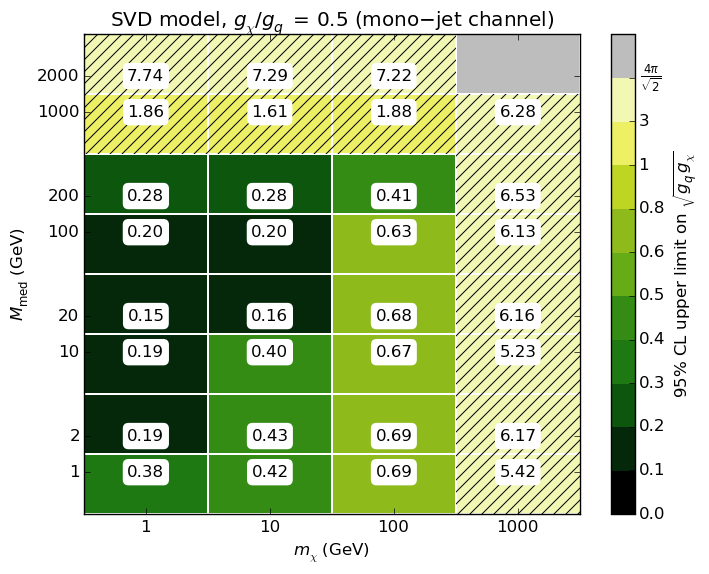
\includegraphics[width=1.\textwidth]{figures/grid_basepoints_SVD_rat05_monojet.png}
      \caption{}
    \end{subfigure}
    \begin{subfigure}[t]{0.495\textwidth}
      \centering
      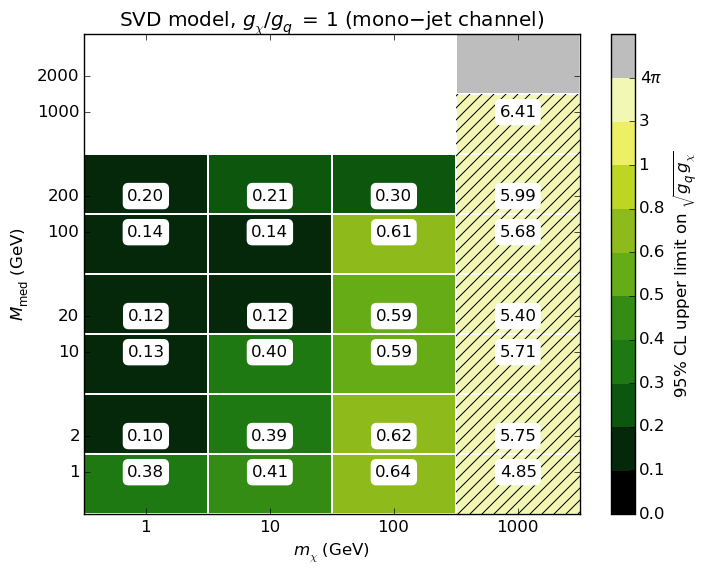
\includegraphics[width=1.\textwidth]{figures/grid_basepoints_SVD_rat1_monojet.png}
      \caption{}
    \end{subfigure}
    \begin{subfigure}[t]{0.495\textwidth}
      \centering
      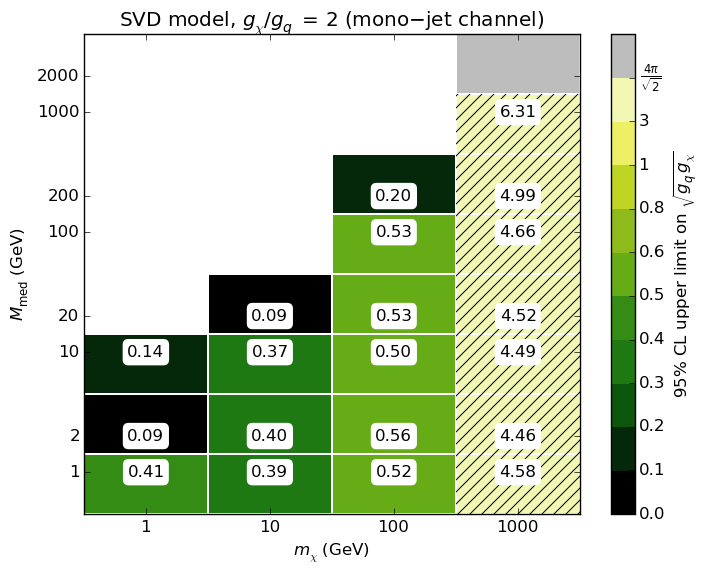
\includegraphics[width=1.\textwidth]{figures/grid_basepoints_SVD_rat2_monojet.png}
      \caption{}
    \end{subfigure}
    \begin{subfigure}[t]{0.495\textwidth}
      \centering
      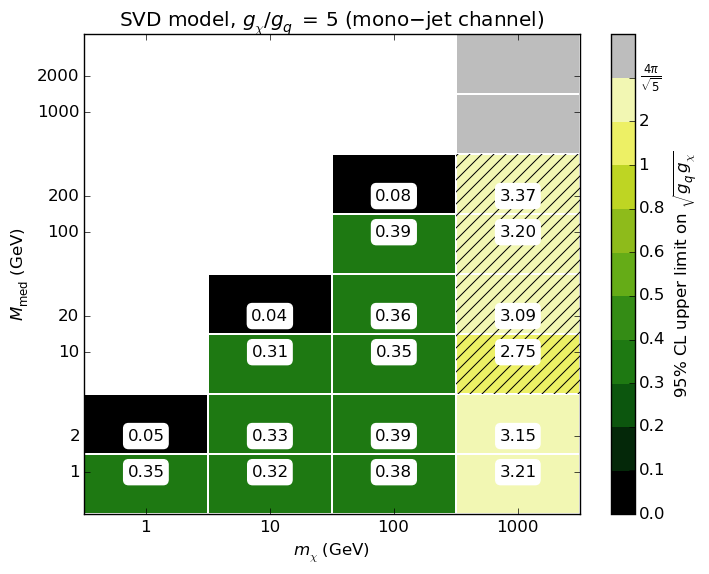
\includegraphics[width=1.\textwidth]{figures/grid_basepoints_SVD_rat5_monojet.png}
      \caption{}
    \end{subfigure}
    \caption{Upper limits on the coupling for the sV model, in the \monojet channel, for $\gX / \gq$ = 0.5 (a), 1 (b), 2 (c) and 5 (d). The grey region represents the phase space where no meaningful limit was obtained. The hatched region represents a limit which leads to a width greater than $\Mmed / 2$, so the validity of the calculation begins to fail.}
    \label{fig:Monojet_SVD_couplinglimit}
\end{figure}

\begin{figure}[h]
  \centering
    \begin{subfigure}[t]{0.495\textwidth}
      \centering
      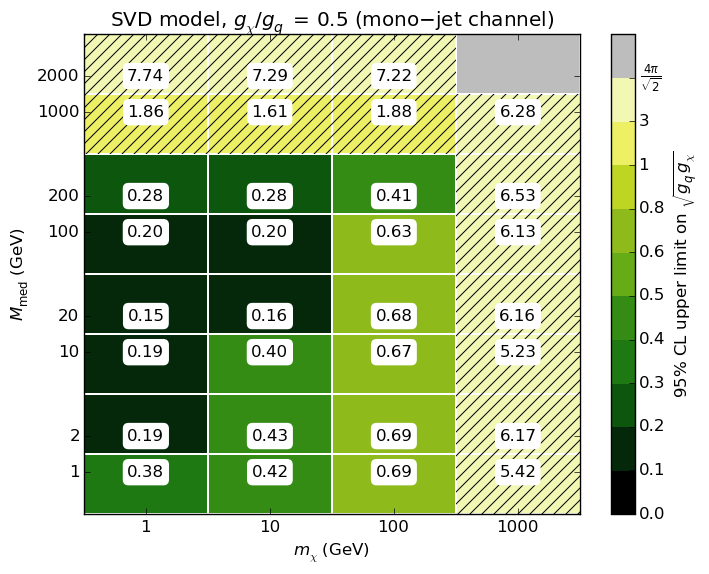
\includegraphics[width=1.\textwidth]{figures/grid_basepoints_SVD_rat05_monojet.png}
      \caption{}
    \end{subfigure}
    \begin{subfigure}[t]{0.495\textwidth}
      \centering
      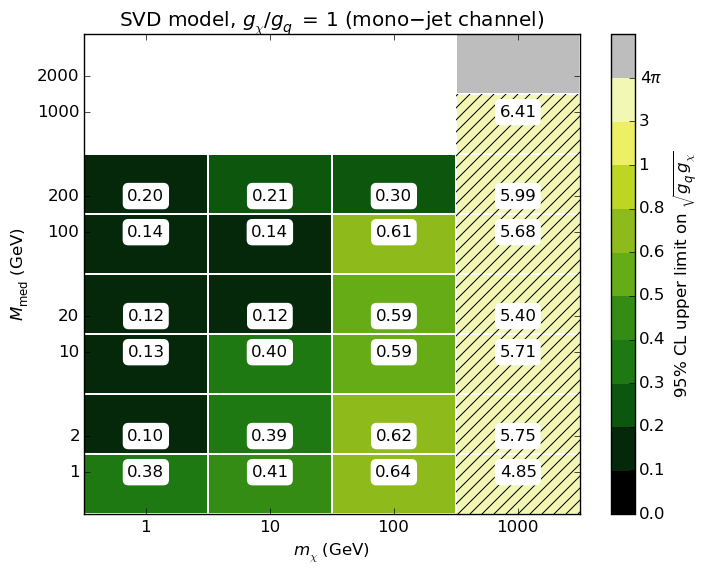
\includegraphics[width=1.\textwidth]{figures/grid_basepoints_SVD_rat1_monojet.png}
      \caption{}
    \end{subfigure}
    \begin{subfigure}[t]{0.495\textwidth}
      \centering
      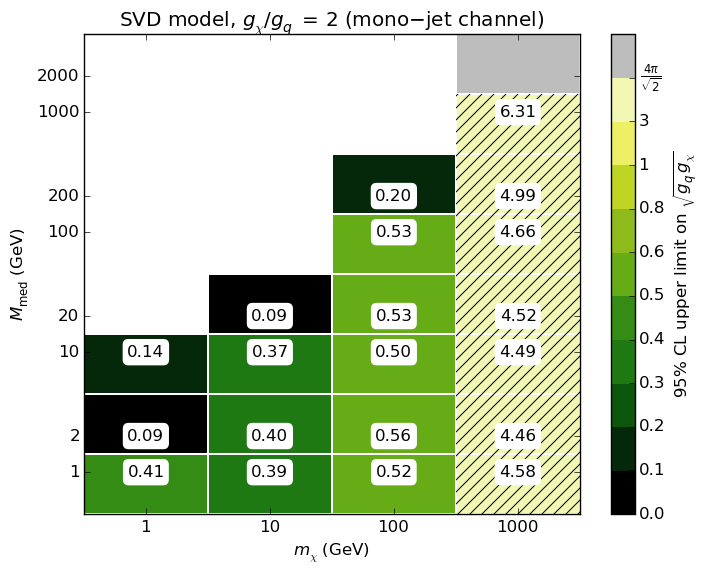
\includegraphics[width=1.\textwidth]{figures/grid_basepoints_SVD_rat2_monojet.png}
      \caption{}
    \end{subfigure}
    \begin{subfigure}[t]{0.495\textwidth}
      \centering
      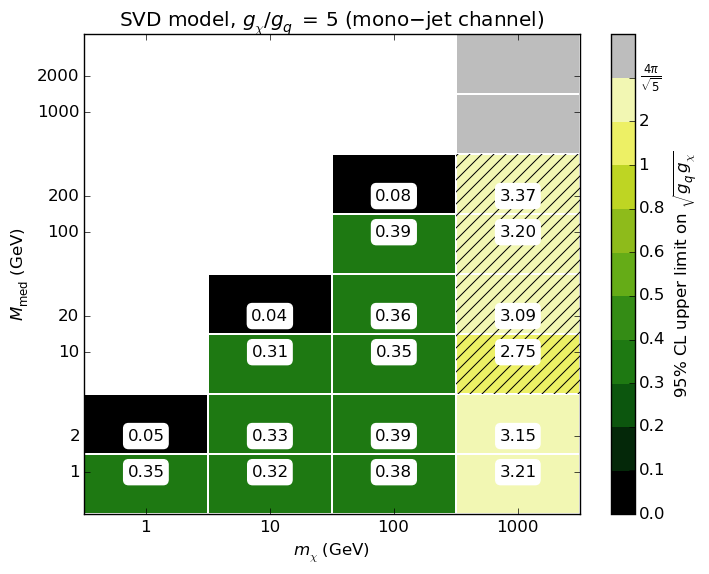
\includegraphics[width=1.\textwidth]{figures/grid_basepoints_SVD_rat5_monojet.png}
      \caption{}
    \end{subfigure}
    \caption{Upper limits on the coupling for the sA model, in the \monojet channel, for $\gX / \gq$ = 0.5 (a), 1 (b), 2 (c) and 5 (d). The grey region represents the phase space where no meaningful limit was obtained. The hatched region represents a limit which leads to a width greater than $\Mmed / 2$, so the validity of the calculation begins to fail. TO BE UPDATED WITH sA PLOTS.}
    \label{fig:Monojet_SVD_couplinglimit}
\end{figure}

Results discussion here.

\subsection{Mono-$Z$ channel}

\begin{figure}[h]
  \centering
    \begin{subfigure}[t]{0.495\textwidth}
      \centering
      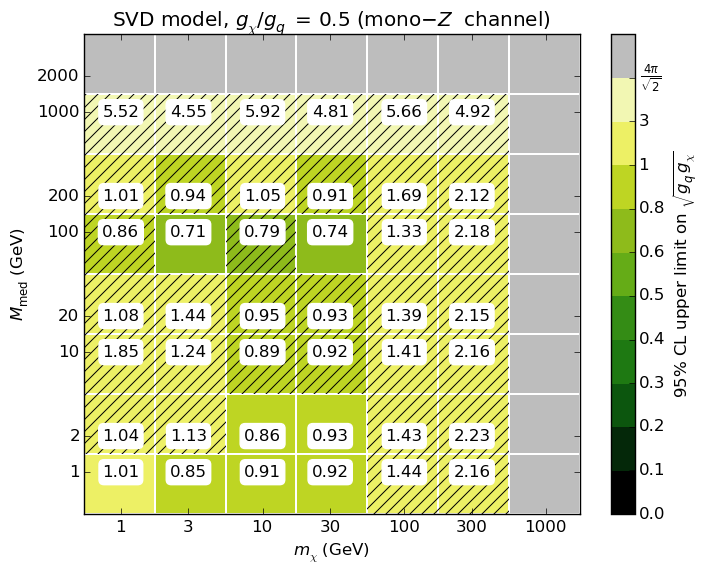
\includegraphics[width=1.\textwidth]{figures/grid_allpoints_SVD_rat05.png}
      \caption{}
    \end{subfigure}
    \begin{subfigure}[t]{0.495\textwidth}
      \centering
      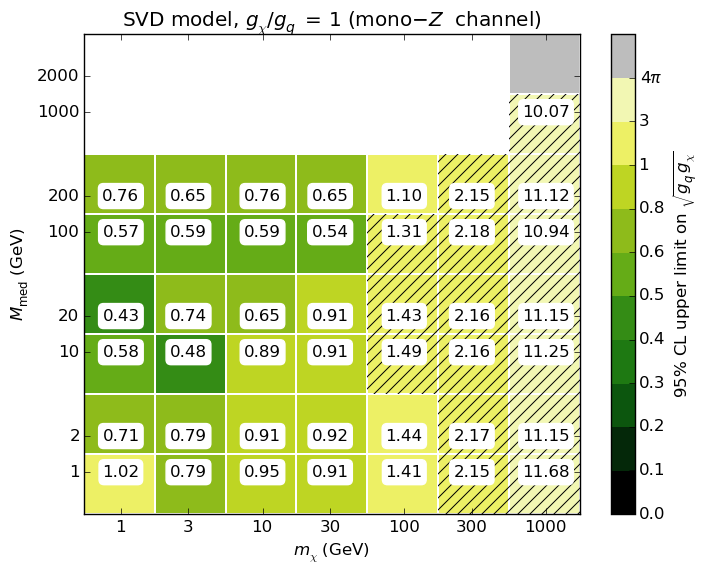
\includegraphics[width=1.\textwidth]{figures/grid_allpoints_SVD_rat1.png}
      \caption{}
    \end{subfigure}
    \begin{subfigure}[t]{0.495\textwidth}
      \centering
      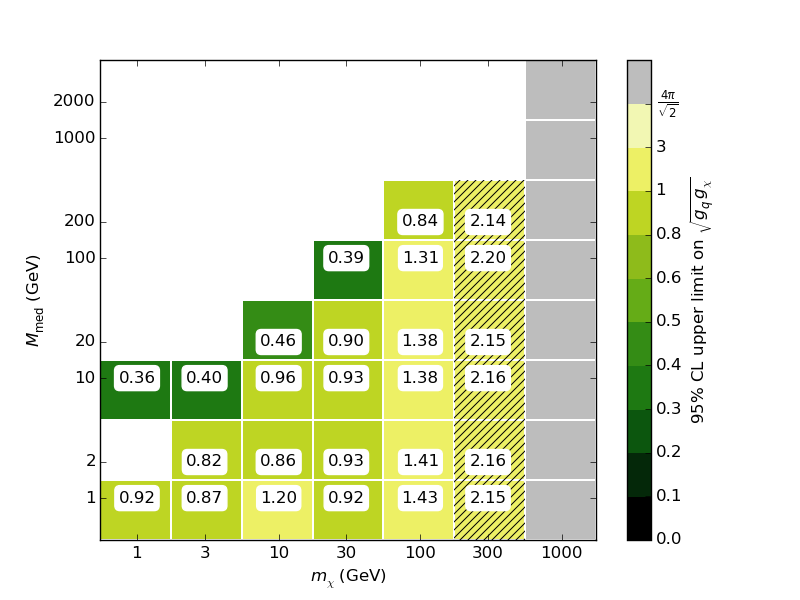
\includegraphics[width=1.\textwidth]{figures/grid_allpoints_SVD_rat2.png}
      \caption{}
    \end{subfigure}
    \begin{subfigure}[t]{0.495\textwidth}
      \centering
      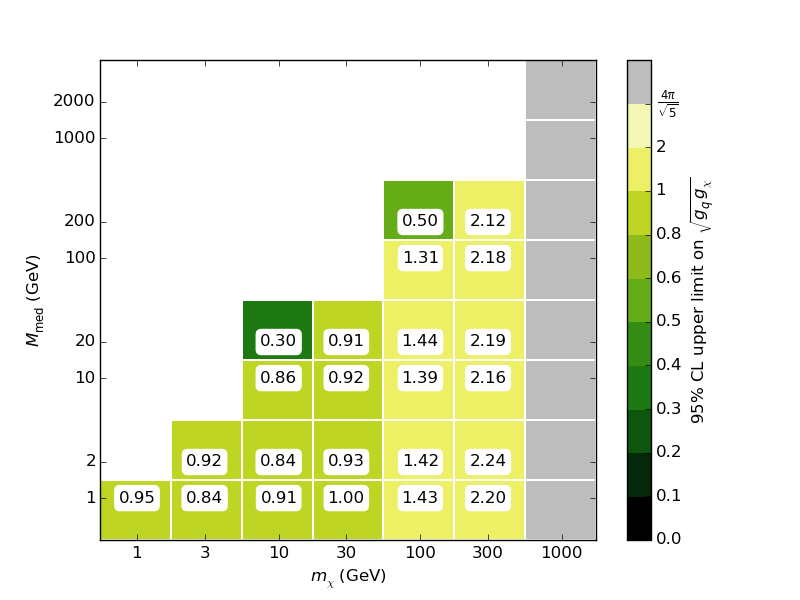
\includegraphics[width=1.\textwidth]{figures/grid_allpoints_SVD_rat5.png}
      \caption{}
    \end{subfigure}
    \caption{Upper limits on the coupling for the sV model, in the \monoZ channel, for $\gX / \gq$ = 0.5 (a), 1 (b), 2 (c) and 5 (d). The grey region represents the phase space where no meaningful limit was obtained. The hatched region represents a limit which leads to a width greater than $\Mmed / 2$, so the validity of the calculation begins to fail.}
    \label{fig:MonoZ_SVD_couplinglimit}
\end{figure}

\begin{figure}[h]
  \centering
    \begin{subfigure}[t]{0.495\textwidth}
      \centering
      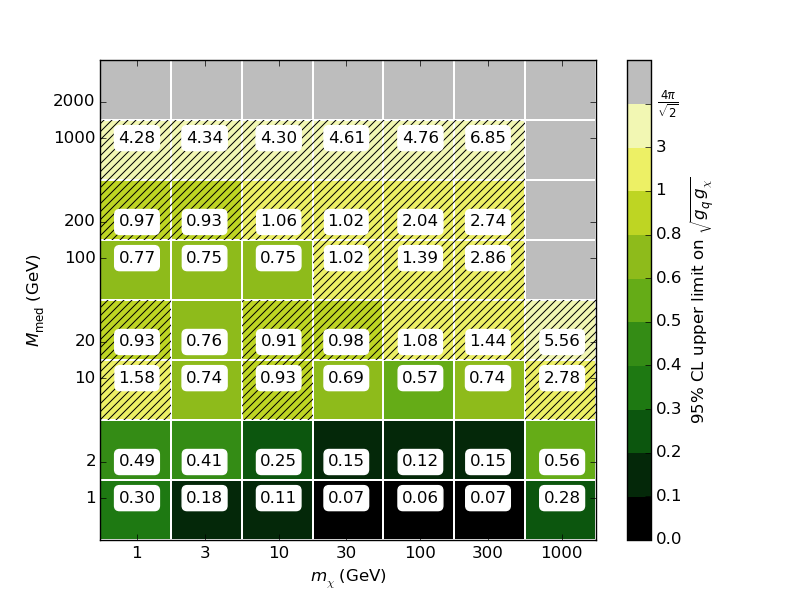
\includegraphics[width=1.\textwidth]{figures/grid_allpoints_SAD_rat05.png}
      \caption{}
    \end{subfigure}
    \begin{subfigure}[t]{0.495\textwidth}
      \centering
      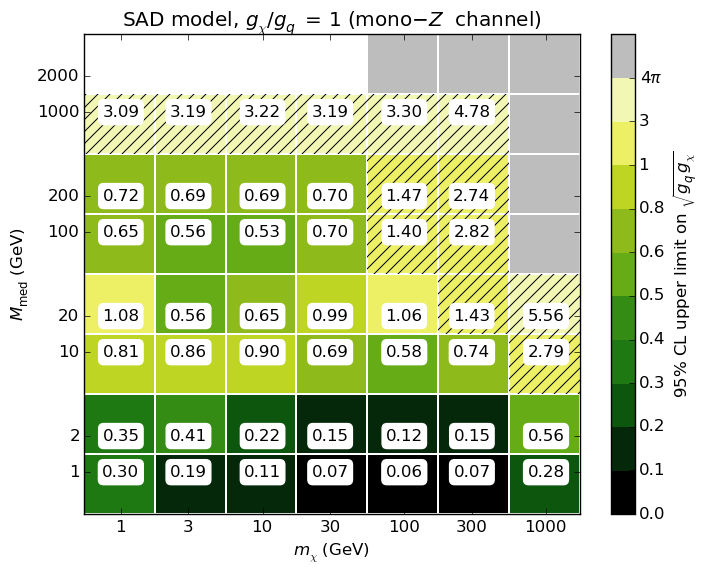
\includegraphics[width=1.\textwidth]{figures/grid_allpoints_SAD_rat1.png}
      \caption{}
    \end{subfigure}
    \begin{subfigure}[t]{0.495\textwidth}
      \centering
      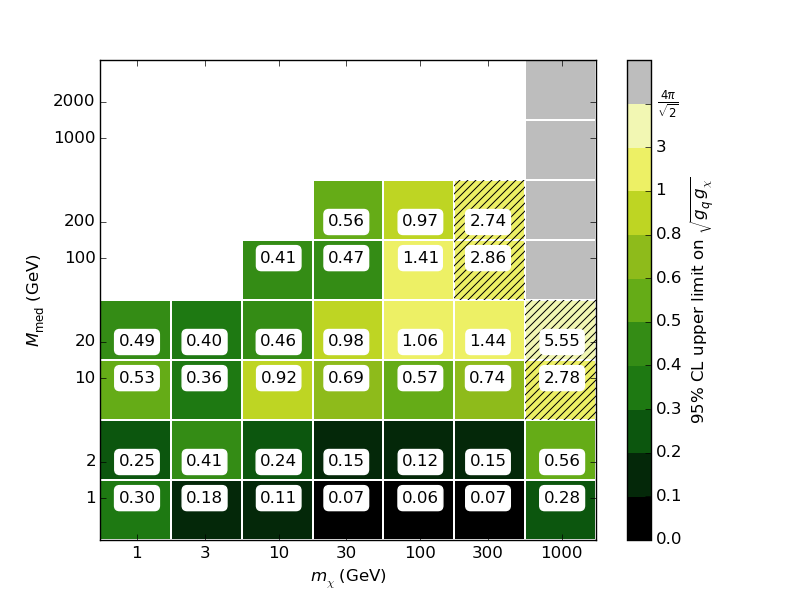
\includegraphics[width=1.\textwidth]{figures/grid_allpoints_SAD_rat2.png}
      \caption{}
    \end{subfigure}
    \begin{subfigure}[t]{0.495\textwidth}
      \centering
      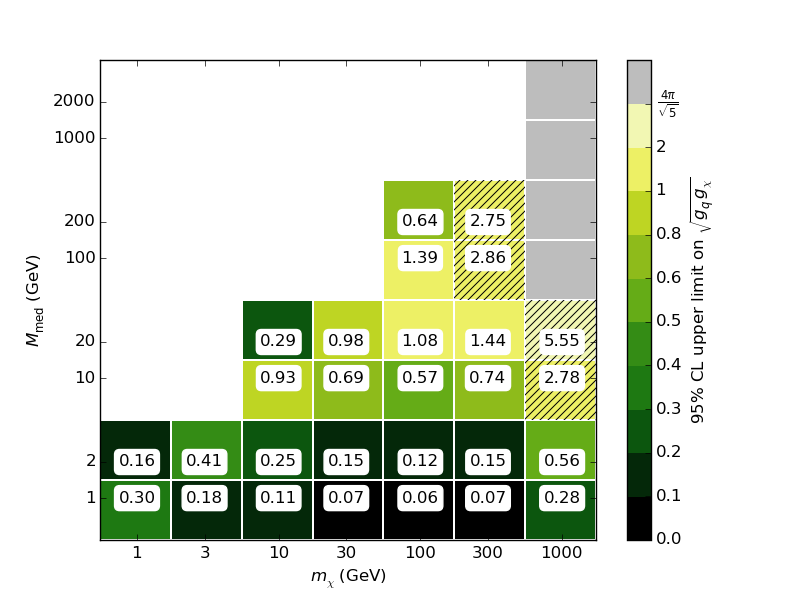
\includegraphics[width=1.\textwidth]{figures/grid_allpoints_SAD_rat5.png}
      \caption{}
    \end{subfigure}
    \caption{Upper limits on the coupling for the sA model, in the \monoZ channel, for $\gX / \gq$ = 0.5 (a), 1 (b), 2 (c) and 5 (d). The grey region represents the phase space where no meaningful limit was obtained. The hatched region represents a limit which leads to a width greater than $\Mmed / 2$, so the validity of the calculation begins to fail.}
    \label{fig:MonoZ_SAD_couplinglimit}
\end{figure}

\begin{figure}[h]
  \centering
    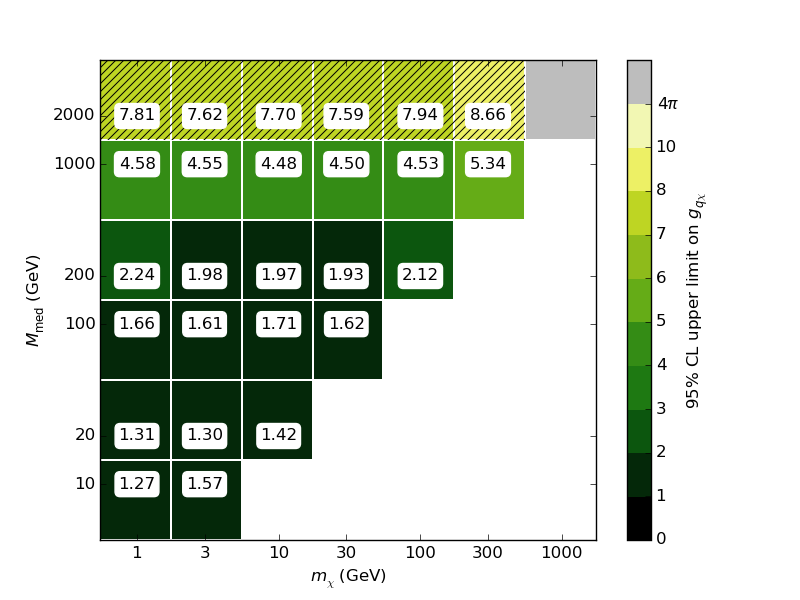
\includegraphics[width=0.6\textwidth]{figures/grid_allpoints_TSD_rat1.png}
    \caption{Upper limit on the coupling $\gqX$ for the tS model, in the \monoZ channel. The grey region represents the phase space where no meaningful limit was obtained. The hatched region represents a limit which leads to a width greater than $\Mmed / 2$, so the validity of the calculation begins to fail.}
    \label{fig:MonoZ_TSD_couplinglimit}
\end{figure}

Mono-Z limits discussion here. Overall uncertainty on $\sqrtgqgX$ generally $ < 10\%$, up to 80$\%$. Large DM masses: small cross sections, limited by ATLAS analysis optimisation, requires more data or further optimisation. Small DM masses: have low $\met$, would require more statistics.

\subsection{Mono-$W/Z$ channel}

\begin{figure}[h]
  \centering
    \begin{subfigure}[t]{0.495\textwidth}
      \centering
      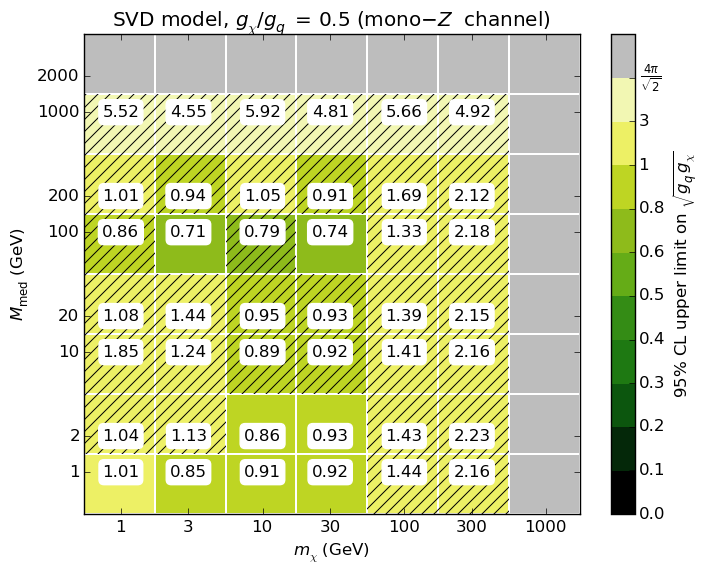
\includegraphics[width=1.\textwidth]{figures/grid_allpoints_SVD_rat05.png}
      \caption{}
    \end{subfigure}
    \begin{subfigure}[t]{0.495\textwidth}
      \centering
      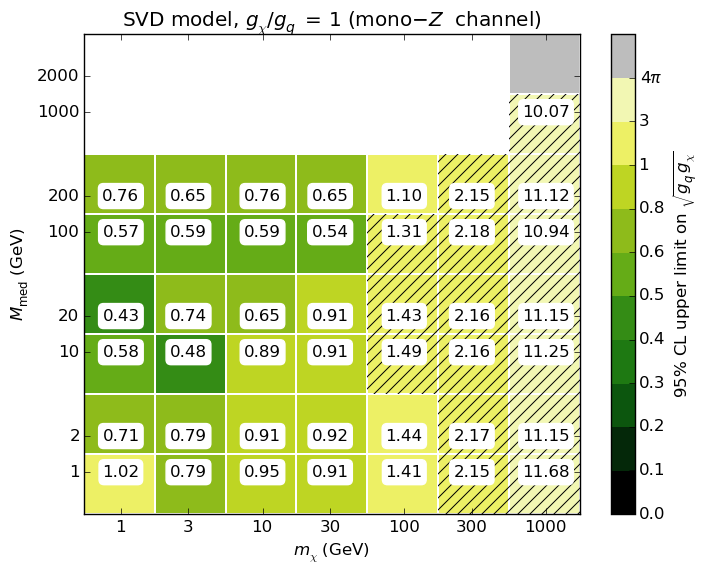
\includegraphics[width=1.\textwidth]{figures/grid_allpoints_SVD_rat1.png}
      \caption{}
    \end{subfigure}
    \begin{subfigure}[t]{0.495\textwidth}
      \centering
      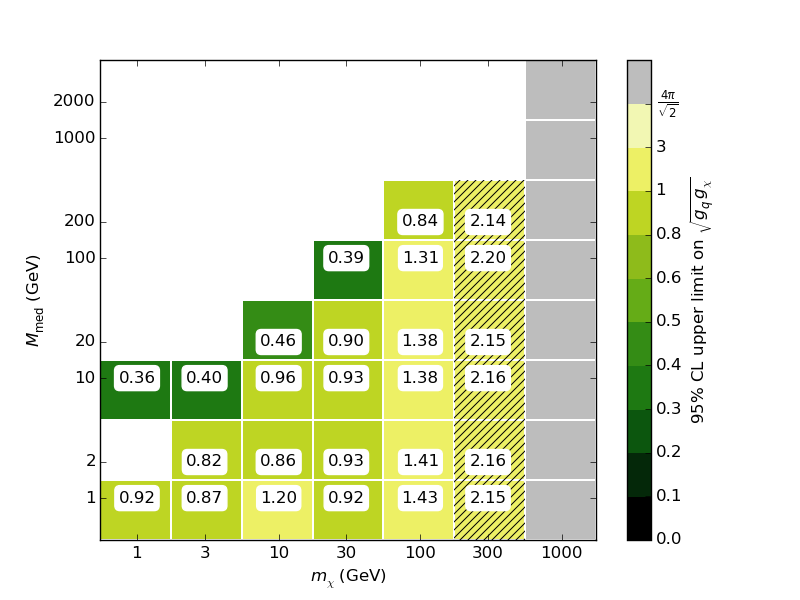
\includegraphics[width=1.\textwidth]{figures/grid_allpoints_SVD_rat2.png}
      \caption{}
    \end{subfigure}
    \begin{subfigure}[t]{0.495\textwidth}
      \centering
      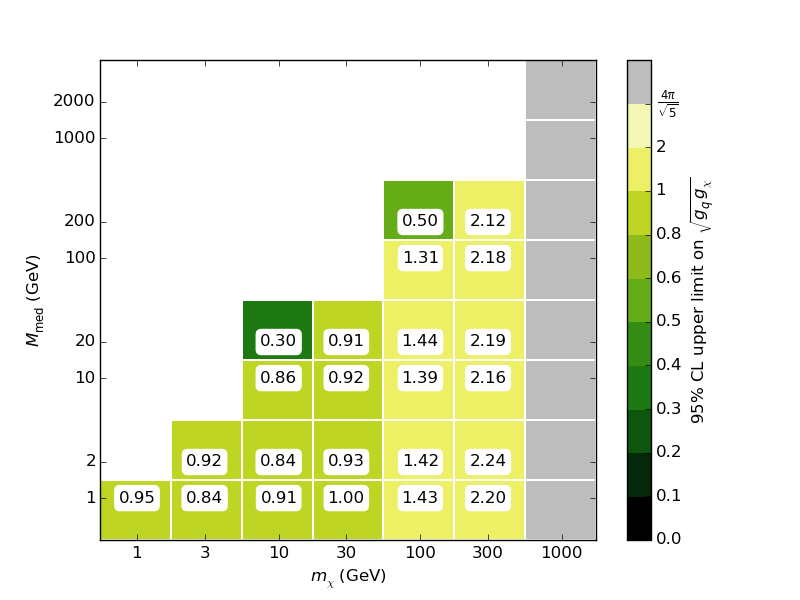
\includegraphics[width=1.\textwidth]{figures/grid_allpoints_SVD_rat5.png}
      \caption{}
    \end{subfigure}
    \caption{Upper limits on the coupling for the sV model, in the \monoWZ channel, for $\gX / \gq$ = 0.5 (a), 1 (b), 2 (c) and 5 (d). The grey region represents the phase space where no meaningful limit was obtained. The hatched region represents a limit which leads to a width greater than $\Mmed / 2$, so the validity of the calculation begins to fail. TO BE UPDATED WITH MONOWZ PLOTS.}
    \label{fig:MonoWZ_SVD_couplinglimit}
\end{figure}

\begin{figure}[h]
  \centering
    \begin{subfigure}[t]{0.495\textwidth}
      \centering
      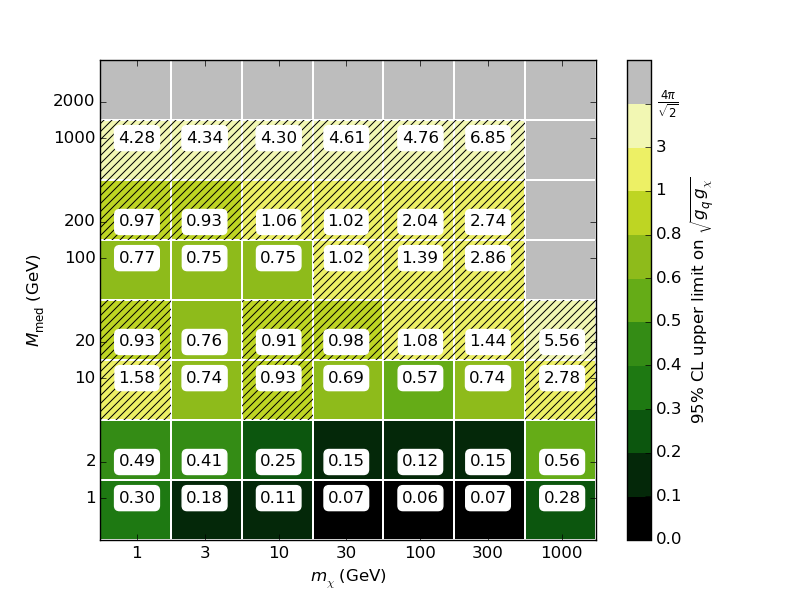
\includegraphics[width=1.\textwidth]{figures/grid_allpoints_SAD_rat05.png}
      \caption{}
    \end{subfigure}
    \begin{subfigure}[t]{0.495\textwidth}
      \centering
      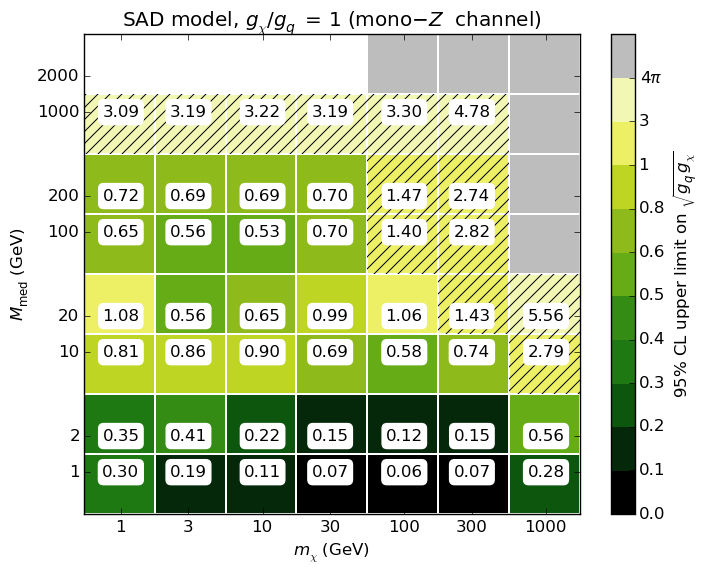
\includegraphics[width=1.\textwidth]{figures/grid_allpoints_SAD_rat1.png}
      \caption{}
    \end{subfigure}
    \begin{subfigure}[t]{0.495\textwidth}
      \centering
      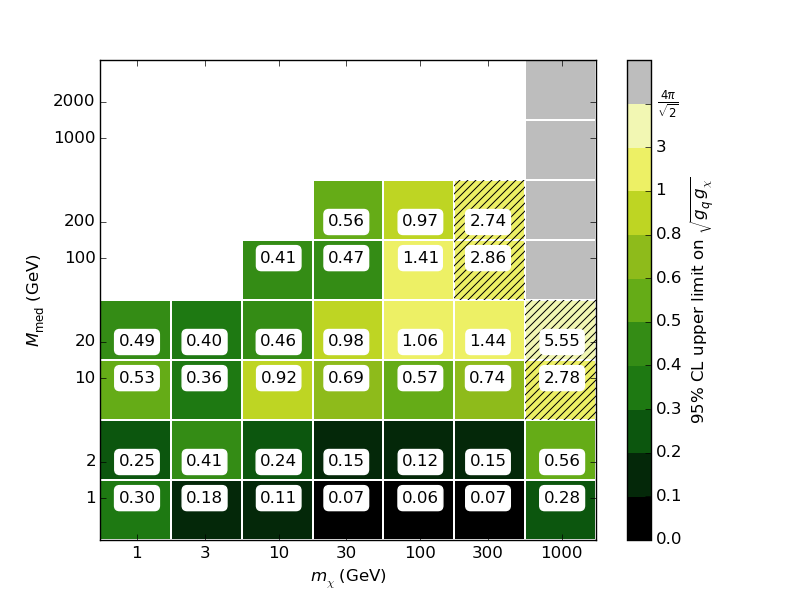
\includegraphics[width=1.\textwidth]{figures/grid_allpoints_SAD_rat2.png}
      \caption{}
    \end{subfigure}
    \begin{subfigure}[t]{0.495\textwidth}
      \centering
      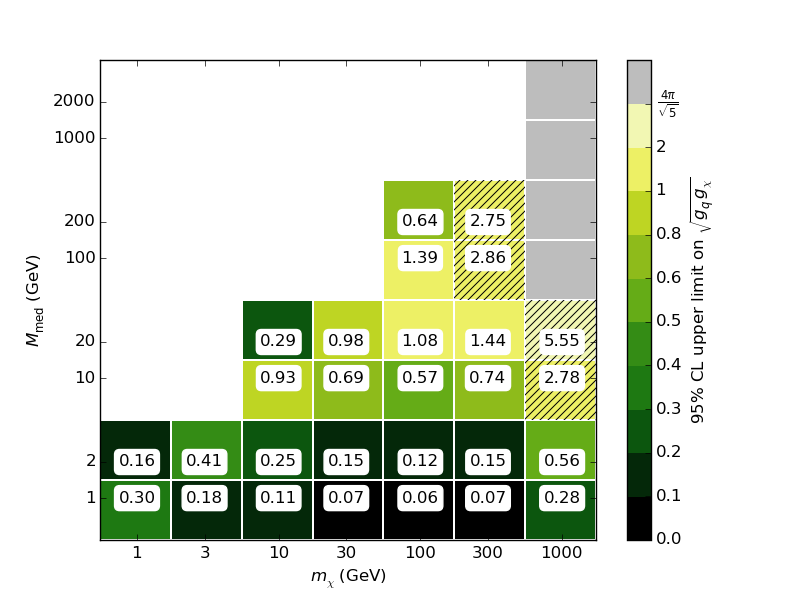
\includegraphics[width=1.\textwidth]{figures/grid_allpoints_SAD_rat5.png}
      \caption{}
    \end{subfigure}
    \caption{Upper limits on the coupling for the sA model, in the \monoWZ channel, for $\gX / \gq$ = 0.5 (a), 1 (b), 2 (c) and 5 (d). The grey region represents the phase space where no meaningful limit was obtained. The hatched region represents a limit which leads to a width greater than $\Mmed / 2$, so the validity of the calculation begins to fail. TO BE UPDATED WITH MONOWZ PLOTS.}
    \label{fig:MonoWZ_SAD_couplinglimit}
\end{figure}

\begin{figure}[!h]
  \centering
    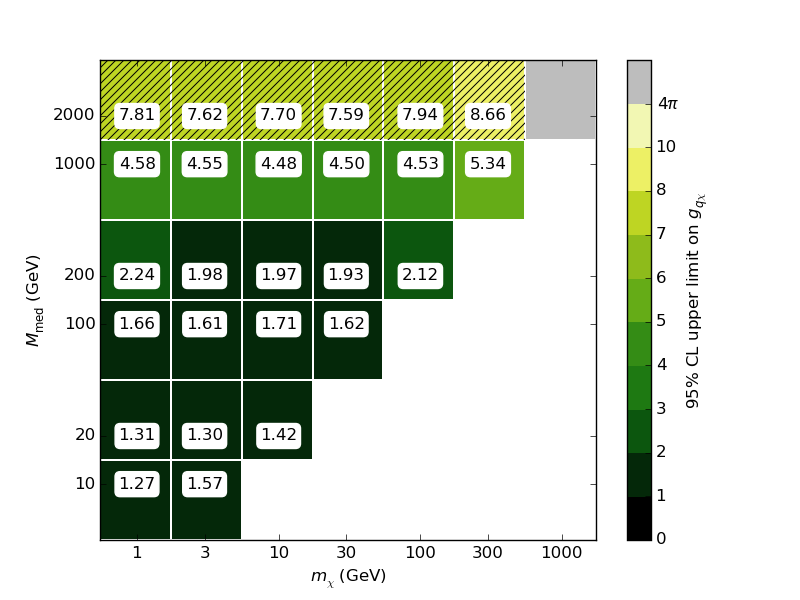
\includegraphics[width=0.6\textwidth]{figures/grid_allpoints_TSD_rat1.png}
    \caption{Upper limit on the coupling $\gqX$ for the tS model, in the \monoWZ channel. The grey region represents the phase space where no meaningful limit was obtained. The hatched region represents a limit which leads to a width greater than $\Mmed / 2$, so the validity of the calculation begins to fail. TO BE UPDATED WITH MONOWZ PLOTS.}
    \label{fig:MonoWZ_TSD_couplinglimit}
\end{figure}

Mono-W/Z limits discussion here.
